\documentclass[journal]{..//IEEEtran/IEEEtran}
\usepackage{cite}
\usepackage[pdftex]{graphicx}
\usepackage{amsmath}
\usepackage{algorithmic}
\usepackage{array}
\usepackage[utf8]{inputenc}
\usepackage{float}
\usepackage{amsmath}
\usepackage{hyperref}
\usepackage[usenames]{color}
\usepackage{microtype}



\begin{document}

\title{Proyecto Inteligencia Artificial\\Primer informe}

\author{Juan Fernando Angulo, Camilo Escobar Arteaga, Danna García Trujillo, Camilo Gutiérrez Córdoba, Andrea Núñez Rodríguez}
\markboth{Proyecto de inteligencia artificial,~Reporte No.~1}
{Shell \MakeLowercase{\textit{et al.}}: Documentación}

\maketitle


\section{Preguntas de interés}


\begin{itemize}
    \item ¿El año de fabricación de los autos y la cantidad de puertas es determinante en el precio final de ventas? Intención: Responder esta pregunta sería de gran ayuda a la hora de comprender el dominio del problema, las correlaciones entre sus variables y características de trasfondo.
    \item ¿En qué zonas del país se presenta un mayor nivel de adquisición de autos usados? Intención: Realizamos esta pregunta nos ayuda a entender de qué forma afecta las regiones geográficas en la venta de un auto usado.
    \item ¿De qué forma se ve afectado el precio de venta simulado dado fluctuaciones en el kilometraje del auto a vender? Intención: Responder a esta pregunta nos daría una perspectiva de que tan sensible es la variable de salida a cambios continuos dados por escalar en variables de entrada. 
  
\end{itemize}
\section{Tipo de problema}
El tipo de problema al que pertenece nuestra temática es de regresión, este es un subcampo de aprendizaje automático supervisado cuyo objetivo es establecer un método para la relación entre un cierto número de características es decir una variable X y una variable objetivo Y de tipo continua.  Esto nos permite predecir datos y en este caso los precios de venta de carros usados es decir Y nuestra variable de respuesta, teniendo en cuenta nuestra una variable de entrada X con atributos del carro como marca, modelo, kilometraje, color, etc.. 

\section{Metodología}

Para el desarrollo del proyecto se optó por usar la metodología CRISP-DM (Cross Industry Standar Process for Data Mining) dado que es una metodología que incluye las fases de un proyecto, sus tareas respectivas, y las relaciones entre estas tareas. Durante el desarrollo del proyecto se llevaron a cabo tres de las seis fases de CRISP-DM.

\begin{itemize}
    \item Entendimiento del negocio
    En esta fase inicial se identificaron los objetivos y requisitos del proyecto desde una perspectiva empresarial, para así poder convertir este conocimiento en un problema de minería de datos.
    \item Comprensión de los datos
    Esta fase comienza con la recolección de datos que fueron obtenidos de la página web TuCarro.com de Mercado Libre. A través de la técnica de web-scraping se recolectaron 1976 datos. En esta fase igualmente realizamos la exploración de datos para familiarizarnos con estos e identificar problemas de la calidad de datos. Por medio de esta exploración definimos el tipo de cada dato de los 11 atributos.
    \item Preparación de los datos
    Por medio del análisis exploratorio encontramos 760 datos de tipo nan, se identificaron cuales de los atributos presentaban este problema con el fin de realizar la investigación sobre las formas de solucionar este problema sin recurrir a la eliminación de estos datos. Adicionalmente, por medio de las estadísticas de los atributos encontramos datos atípicos que igualmente se esta considerando la manera de corregirlo por medio de normalización sin acudir a la eliminación de estos datos.

    
\end{itemize}
    



\section{Métricas}

\begin{enumerate}
    \item Error cuadrático medio (MSE) entre las predicciones producidas por el modelo de machine learning en contraste al set de datos de verificación. 
    \item Proporción de error predictivo calculado mediante set de estimaciones de origen netamente humano.
    \item Error porcentual Absoluto (MAPE).
    \item Otras métricas relacionadas directamente al método de machine learning a usar.
\end{enumerate}

\section{Datos recolectados}
Los datos recolectados se obtuvieron a partir de un web scraping a la página de Mercado Libre. Este es un método muy avanzado que es altamente flexible y potente cuando de recolectar información se trata. A partir de esta técnica se recolectaron 1976 datos los cuales contaban con 11 atributos. De esta manera, logramos recoger una serie de atributos importantes de las variables determinantes de un carro al momento de su venta, para así completar nuestro set de datos, estas variables son: la marca, el modelo, el año, el kilometraje, el número de puertas, el tipo de combustible, el motor, la transmisión, el color y el tipo de carrocería.

\section{Análisis exploratorio}

Después de la recolección de los datos se realizó un análisis exploratorio de los mismos, en el cual se evidenciaron algunas características relevantes. El conjunto de datos consta de 10 variables tipadas como sigue:


\begin{tabular}{l l l}
    Variable & Descripción & Tipo \\ \hline
    brand & Marca fabricante & Texto \\
    color & Color del chasis &Texto \\
    doors & Puertas & Texto \\
    fuelType & Tipo de combustible utilizado & Texto \\
    model & Modelo de fabricación & Texto \\
    motor & Tipo de motor & Texto \\
    price & Precio de venta & Numerico \\
    transmission & Tipo de transmisión & Texto \\
    year & Año de fabricación & Numerico 
\end{tabular}\\\\



Al tener el dataset en condiciones óptimas, se hizo un análisis más profundo de cada algunas de sus variables con el objetivos de estudiar su comportamiento. A continuación se puede visualizar algunos de los gráficos que se obtuvieron de este proceso

\begin{figure}[H]
    \centering
    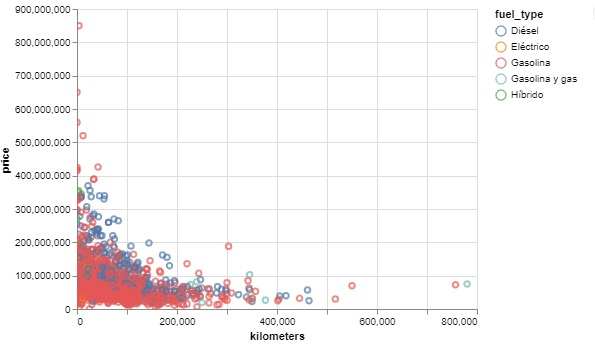
\includegraphics[width=0.5\textwidth]{images/dispersion.jpeg}
    \caption{Gráfico de dispersion de kilometraje y precio coloreado de acuerdo al tipo de combustible }
    \label{diagramaD}
    \end{figure}
\begin{figure}[H]
    \centering
    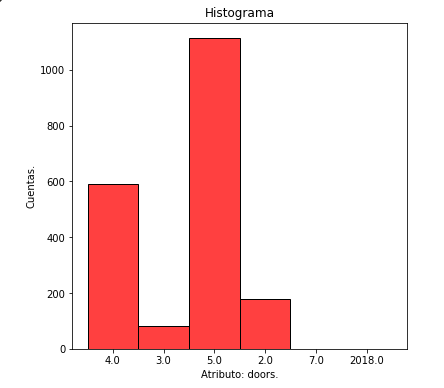
\includegraphics[width=0.5\textwidth]{images/histograma.PNG}
    \caption{Histograma sobre el atributo puertas del carro.}
    \label{histograma1}
\end{figure}



En el gráfico \ref{diagramaD} se puede apreciar el comportamiento de tres variables del dataset, las cuales son el kilometraje, el precio y el color de un carro, esto nos ayuda a analizar qué tan importantes e influyentes son estas propiedades a la hora de vender un auto.

En el gráfico \ref{histograma1} se puede observar qué tan diversos son los tipos de carros que se venden a partir del atributo "puertas". De esta manera podríamos identificar si este atributo puede llegar a ser relevante en el precio de venta de un auto. \\

Recurso: \definecolor{Micolor1}{RGB}{0,0,255}
\textcolor{Micolor1}{\href{https://colab.research.google.com/drive/1JEJDNylgwW9VSxS-4pY8_b2a_9Aqz3Hw?usp=sharin}{Codebook de análisis exploratorio}}

\section{Siguientes pasos}
Investigar formas de rellenar espacios vacíos (NaN) en el dataframe, de forma que no tengamos que eliminar estas filas, y así poder trabajar con una mayor cantidad de datos.\\

Modificar el scraper para que extraiga la ubicación como variable también y recolectar más datos de otras páginas web que vendan carros usados, y luego juntar todos los datos recolectados de distintos sitios en un solo dataframe organizado, para así lograr un mejor entrenamiento del modelo.\\

Desarrollar un modelo que nos permita predecir el precio de venta de un auto usado de acuerdo a unas características seleccionadas, y entrenarlo con los datos recolectados.\\



\hfill Septiembre 19, 2021.


\end{document}